
\documentclass[titlepage, 11pt]{article}
\title{Machine learning: Assignment 2}
\author{Mathias Mellemstuen}
\date{13 October 2021}
\usepackage{times}
\renewcommand{\baselinestretch}{1.5}

\usepackage[margin=1.0in]{geometry}
\usepackage{listings}
\usepackage{color}

\definecolor{dkgreen}{rgb}{0,0.6,0}
\definecolor{gray}{rgb}{0.5,0.5,0.5}
\definecolor{mauve}{rgb}{0.58,0,0.82}

\usepackage{graphicx}
\graphicspath{./}
\lstset{frame=tb,
	language=Python,
	aboveskip=3mm,
	belowskip=3mm,
	showstringspaces=false,
	columns=flexible,
	basicstyle={\small\ttfamily},
	numbers=none,
	numberstyle=\tiny\color{gray},
	keywordstyle=\color{blue},
	commentstyle=\color{dkgreen},
	stringstyle=\color{mauve},
	breaklines=true,
	breakatwhitespace=true,
	tabsize=3
}

\begin{document}
    \maketitle

    \section{Content}
    The content of this report will contain the observations from the results of this assignment. 
    \section{Observations}
    After running the algorithm with different parameters, it resultet in this table with data. The table contains the parameters that were used on the algorithm under each run and the output of the algorithm, the score.
    \begin{table}[h!]
        \label{tab:table1}
        \begin{tabular}{|l|l|l|l|l|}
            \hline
            \textbf{Index} & \textbf{Test Size} & \textbf{Layers and nodes} & \textbf{Max Iterations} & \textbf{Score} \\ \hline
            1 & 0.3 & (100, 50) & 40000 & 97.78\% \\ \hline
            2 & 0.7 & (100, 50) & 40000 & 96.03\% \\ \hline
            3 & 0.3 & (1, ) & 40000 & 8.89\% \\ \hline
            4 & 0.3 & (100, 200, 50, 50), & 40000 & 96.3\% \\ \hline
        \end{tabular}
    \end{table}
    It is clear by reading of the table that the accuracy (score) is higher when the number of layers and nodes are higher. When running the algorithm with only one node and layer, the score is very low at just 8.89\%. The table shows that it only helps to increase the number of nodes and hidden layers to a certain extent. 

    \begin{center}
        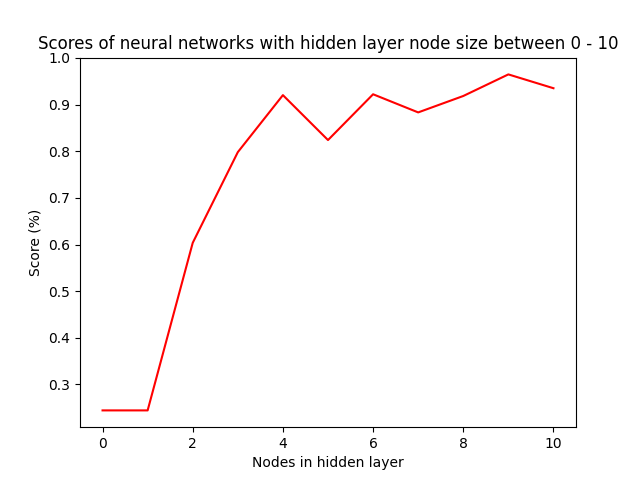
\includegraphics[scale=0.5]{Accuracy-1-10.png}
        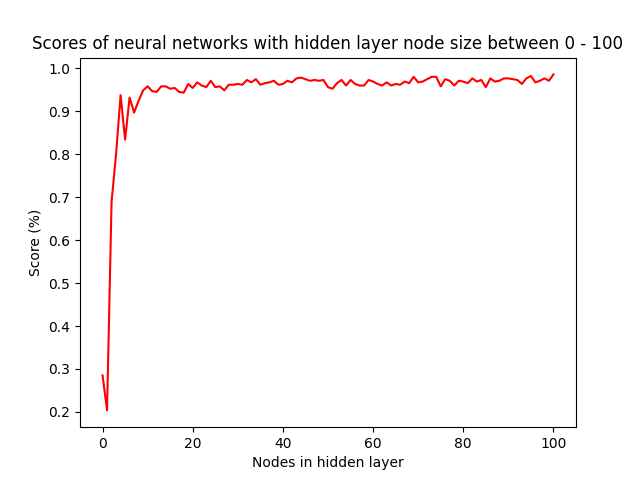
\includegraphics[scale=0.5]{Accuracy-1-100.png}
    \end{center}The next graph at the left side are visualizing exactly what this looks like. The graph has a very high increase between x value 2 and 3. Later, the curve is flattening more and laying between 90\%-100\% accuracy.
    It becomes more clear when looking at the graph at the right side. This graph shows accuracy between 1 - 100 nodes. The graph shows once again that the accuracy are staying between 90\%-100\% after the first few values. The purpose of this graph is showing that it continues to stay in the 90\%-100\% range. After observing these results, it becomes clear that the only way to increase the accuracy further is to increase the number of hidden layers.
    \begin{center}
    \end{center}
\end{document}